\section{Experiment}
\label{sec:experiment}

This section reports two 109B-scale experiments used to validate the final \method{} design on a native multimodal model trained on a mixture of text and image/video data. The first trains a native \method{} model from scratch, which we denote as \textbf{\method{}-PT}. The second starts from a Full-Attention checkpoint and continues pretraining after replacing dense attention with \method{}, which we denote as \textbf{\method{}-CPT}. Both models use the same architecture family as the Full-Attention baseline, but replace dense attention with the \method{} layer.


\subsection{Setup}
\label{sec:experiment-setup}

\paragraph{Model Structure.} All models use the same 41-layer MoE backbone, with approximately 109B total parameters and 6B activated parameters per token. The first three layers are dense layers, and the remaining 38 layers are MoE layers. The model uses a 200K-token vocabulary and hidden size $d_{\rm model}=3072$. Each attention module uses MSA with 64 query heads, 4 KV heads, head dimension 128, and RoPE dimension 64. Each MoE layer uses 128 routed experts, 1 shared expert, and top-4 routed expert selection. During sparse training and evaluation, both \method{} models use block size \(B_k=128\) and keep \(k=16\) key-value blocks per query and GQA group.

\paragraph{Training Budget.} All models are trained under a total budget of 3T tokens. \method{}-PT is trained from scratch: after a 40B-token indexer warmup, it remains in sparse training for the rest of pretraining. \method{}-CPT starts from a GQA Full-Attention checkpoint trained on 2.6T tokens. We then replace dense attention with \method{} and continue training for 400B tokens: the first 40B tokens are used for indexer warmup, followed by sparse continued pretraining.

\paragraph{Evaluations.} We evaluate Full, \method{}-PT, and \method{}-CPT on the same pretraining evaluation suite using matched checkpoints under the same training budget. For general reasoning and question answering, we use MMLU~\citep{hendrycks2021measuring}, MMLU-Pro~\citep{NEURIPS2024_ad236edc}, BBH~\citep{suzgun2022challengingbigbenchtaskschainofthought}, GPQA Hard~\citep{rein2023gpqa}, ARC Challenge~\citep{clark2018thinksolvedquestionanswering}, TriviaQA~\citep{joshi-etal-2017-triviaqa}, and WinoGrande~\citep{Sakaguchi_2020}. For math and code, we use GSM8K~\citep{cobbe2021trainingverifierssolvemath}, MGSM~\citep{shi2022languagemodelsmultilingualchainofthought}, MathVista~\citep{lu2024mathvista}, OlymMATH~\citep{sun2025olymmath}, HumanEval~\citep{chen2021evaluatinglargelanguagemodels}, EvalPlus~\citep{NEURIPS2023_43e9d647}, BigCodeBench~\citep{zhuo2025bigcodebench}, and MultiPL-E MBPP~\citep{cassano2023multipl}. We also evaluate multimodal capability: image benchmarks include AI2D~\citep{kembhavi2016ai2d}, ChartQA~\citep{masry-etal-2022-chartqa}, MMMU~\citep{yue2024mmmu}, OCRBench v2~\citep{fu2025ocrbenchv2improvedbenchmark}, CharXiv~\citep{wang2024charxiv}, VisualWebBench~\citep{liu2024visualwebbench}, and CVBench~\citep{NEURIPS2024_9ee3a664}, while video benchmarks include EgoSchema~\citep{mangalam2023egoschema}, LongVideoBench~\citep{NEURIPS2024_329ad516}, MLVU~\citep{Zhou_2025_CVPR}, MMVU~\citep{zhao2025mmvu}, VideoMME~\citep{fu2024videomme}, and TemporalBench~\citep{cai2024temporalbenchbenchmarkingfinegrainedtemporal}. For long-context evaluation, we use RULER~\citep{hsieh2024ruler} and HELMET~\citep{yen2025helmet}. We additionally report perplexity on downstream agent tasks, including $\tau^2$-bench~\citep{barres2025tau2}, TheAgentCompany~\citep{xu2024theagentcompany}, Humanity's Last Exam~\citep{phan2025hle}, and SWE-bench~\citep{jimenez2024swebench}.


\subsection{Training Dynamics}
\label{sec:experiment-training-dynamics}

\Figref{fig:training-dynamics-pt} compares native sparse pretraining with the matched full-attention run. Over the 3T-token training process, the two LM-loss curves are nearly indistinguishable, showing that \method{} does not introduce noticeable optimization degradation relative to full attention. The gradient-norm curves also remain within the same range throughout training, suggesting that \method{} does not lead to abnormal gradient fluctuations or training instability. These results indicate that training a sparse attention model is as stable as training the full-attention baseline at a large scale.

\Figref{fig:training-dynamics-cpt} illustrates the transition from a trained full-attention checkpoint to sparse continued pretraining. The indexer-warmup stage rapidly reduces the KL loss before sparse attention is enabled. After switching to sparse CPT, the KL loss remains low.
For each query and GQA head, let $\gI^\star$ be the corresponding Top-$k$ block set induced by the Main Branch scores and let $\widehat{\gI}$ be the Index Branch selection. Block recall is $|\gI^\star\cap\widehat{\gI}|/|\gI^\star|$, while score recall is $\sum_{b\in\gI^\star\cap\widehat{\gI}} P_b/\sum_{b\in\gI^\star} P_b$, where $P_b$ is the Main Branch attention probability summed over tokens in block $b$. 
The block recall stays favorable, indicating reliable recovery of important blocks. The higher score recall further shows that the retrieved blocks account for most of the Main Branch attention mass.
Together, these dynamics show that warmup provides a clean conversion phase and that the CPT indexer remains well aligned during sparse continued pretraining.

\begin{figure}[H]
\centering
\begin{subfigure}[t]{0.48\linewidth}
  \centering
  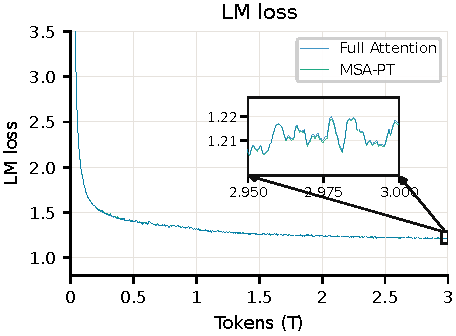
\includegraphics[width=0.84\linewidth]{figures/training_lm_loss_fromscratch_vs_full.pdf}
  \caption{LM loss.}
\end{subfigure}\hfill%
\begin{subfigure}[t]{0.48\linewidth}
  \centering
  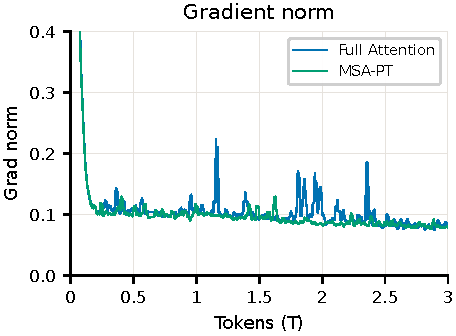
\includegraphics[width=0.84\linewidth]{figures/training_grad_norm_fromscratch_vs_full.pdf}
  \caption{Gradient norm.}
\end{subfigure}
\caption{Pretraining dynamics for the experiment model. LM loss and gradient norm are shown for Full Attention and \method{}-PT over 3T training tokens. The inset in (a) zooms in on the final 50B-token window, where the two LM-loss curves remain nearly overlapping.}
\label{fig:training-dynamics-pt}
\end{figure}

\begin{figure}[H]
\centering
\begin{subfigure}[t]{0.48\linewidth}
  \centering
  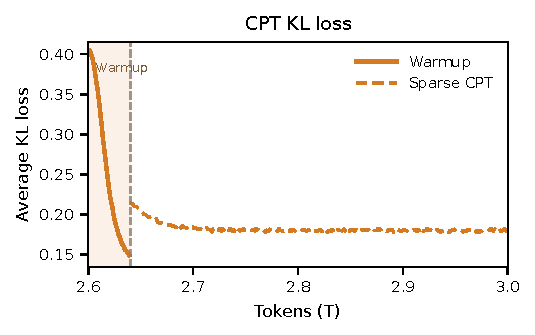
\includegraphics[width=0.84\linewidth]{figures/training_kl_loss_cpt_sparse.pdf}
  \caption{KL loss.}
\end{subfigure}\hfill
\begin{subfigure}[t]{0.48\linewidth}
  \centering
  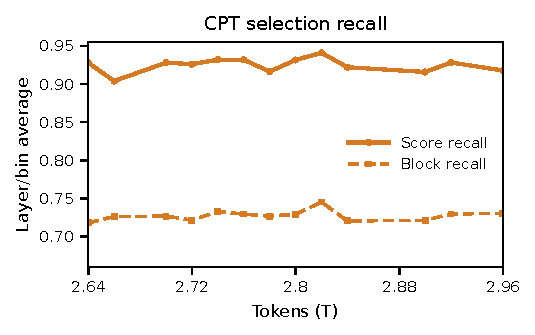
\includegraphics[width=0.84\linewidth]{figures/training_selection_recall_cpt_sparse.pdf}
  \caption{Selection recall.}
\end{subfigure}
\caption{Sparse continued-pretraining dynamics. (a) Average KL loss during \method{}-CPT. The solid segment denotes indexer warmup, and the dashed segment denotes sparse continued pretraining; the vertical dashed line marks the switch between the two stages. (b) Average block recall and score recall of the \method{}-CPT indexer during sparse continued pretraining.}
\label{fig:training-dynamics-cpt}
\end{figure}

\subsection{Main Results}
\label{sec:experiment-main-results}

\Tabref{tab:pretrain-representative} compares Full, \method{}-PT, and \method{}-CPT on a representative set of pretraining evaluations. Both sparse models remain broadly competitive with the Full-Attention baseline, indicating that replacing dense attention with \method{} does not substantially degrade the model's general language, reasoning, multimodal, or agent-oriented perplexity profile. The two training routes show different strengths. \method{}-PT, which learns the sparse pattern throughout pretraining, obtains the strongest results on many math, image, video, and long-context retrieval benchmarks, suggesting that native sparse pretraining can adapt the model representations to the sparse attention pattern. \method{}-CPT is more conservative: it preserves much of the Full-Attention checkpoint behavior and remains close on most text, code, and PPL evaluations, making it a practical conversion route when a trained dense checkpoint is already available. The remaining gaps are benchmark-dependent rather than concentrated in a single capability area.


\begin{table}[H]
\centering
\caption{Representative evaluation results under the 3T-token training budget. Full denotes the Full-Attention baseline, \method{}-PT denotes from-scratch sparse pretraining, and \method{}-CPT denotes sparse continued pretraining. Best per-row results are bolded; lower is better for PPL and higher is better otherwise.}
\label{tab:pretrain-representative}
{\small
\renewcommand{\arraystretch}{0.92}
\begin{adjustbox}{max width=0.95\linewidth}
\begin{tabular}{llrrr}
\toprule
Group & Benchmark & Full & \method{}-PT & \method{}-CPT \\
\midrule
\multirow{7}{*}{\textit{General}} & MMLU & 67.0 & \textbf{67.2} & 66.8 \\
 & MMLU-Pro & 38.5 & 38.8 & \textbf{39.1} \\
 & BBH & \textbf{67.7} & 66.6 & 66.1 \\
 & GPQA Hard & 25.9 & \textbf{26.3} & \textbf{26.3} \\
 & ARC Challenge & 82.7 & 82.5 & \textbf{82.9} \\
 & TriviaQA & 66.0 & 65.5 & \textbf{67.7} \\
 & WinoGrande & 58.3 & 60.9 & \textbf{62.0} \\
\midrule
\multirow{4}{*}{\textit{Math}} & GSM8K & 76.2 & \textbf{77.7} & 73.7 \\
 & MGSM & 44.1 & \textbf{46.0} & 44.2 \\
 & MathVista & 43.8 & \textbf{46.8} & 44.5 \\
 & OlymMATH Easy P@100 & 23.0 & \textbf{26.0} & 22.0 \\
\midrule
\multirow{4}{*}{\textit{Code}} & HumanEval & 61.0 & \textbf{64.0} & 57.9 \\
 & EvalPlus & 59.4 & \textbf{61.8} & 60.0 \\
 & BigCodeBench & 44.8 & 44.0 & \textbf{45.7} \\
 & MultiPL-E MBPP P@10 & \textbf{82.1} & 81.6 & 81.1 \\
\midrule
\multirow{2}{*}{\textit{Retrieval}} & RULER-8K & 79.8 & \textbf{84.2} & 77.2 \\
 & RULER-32K & 75.0 & \textbf{77.5} & 75.7 \\
\midrule
\multirow{7}{*}{\textit{Image}} & AI2D & 68.3 & \textbf{70.6} & 67.3 \\
 & ChartQA & 75.0 & \textbf{75.4} & 71.4 \\
 & MMMU & \textbf{46.8} & 45.9 & 44.5 \\
 & OCRBench v2 & 55.0 & \textbf{55.7} & 54.3 \\
 & CharXiv & 37.55 & \textbf{41.55} & 37.15 \\
 & VisualWebBench & 55.6 & \textbf{68.4} & 59.4 \\
 & CVBench & 57.0 & \textbf{59.7} & 58.8 \\
\midrule
\multirow{6}{*}{\textit{Video}} & EgoSchema & 29.6 & \textbf{37.6} & 25.8 \\
 & LongVideoBench & 38.5 & \textbf{41.8} & 38.9 \\
 & MLVU & 44.14 & \textbf{46.94} & 43.68 \\
 & MMVU & 45.8 & \textbf{47.5} & 45.8 \\
 & VideoMME & 41.11 & \textbf{45.48} & 39.65 \\
 & TemporalBench & 49.4 & \textbf{53.4} & 50.6 \\
\midrule
\multirow{4}{*}{\textit{PPL $\downarrow$}} & TAU2 & 1.155 & \textbf{1.148} & 1.150 \\
 & AgentCompany & 1.248 & 1.249 & \textbf{1.247} \\
 & HLE & \textbf{1.275} & 1.278 & \textbf{1.275} \\
 & SWE & \textbf{1.216} & 1.218 & \textbf{1.216} \\
\bottomrule
\end{tabular}
\end{adjustbox}
}
\end{table}


To evaluate whether \method{} remains effective after long-context scaling, we conduct an additional extension experiment on the \method{}-CPT model. Starting from the sparse continued-pretraining checkpoint, we run approximately 140B tokens of long-context training and then evaluate on HELMET and RULER. The results are reported in \Tabref{tab:lctx-main}. After the extension stage, \method{}-CPT remains close to the Full-Attention baseline. Since each query and GQA group still attends to only \(k B_k=16\times128=2{,}048\) key-value tokens, these results indicate that \method{} can preserve long-context capability under a highly tight attention budget.

Additional ablations supporting these design choices are provided in the appendix. In particular, \Secref{app:prelim} studies the training recipe for the Index Branch, including gradient sources, KL-gradient detachment, warmup, and the comparison with a sliding-window sparse baseline. \Secref{app:additional-ablation} further examines architectural choices such as block size, forced sink, local selection, and the Index Branch value head. These ablations provide the empirical basis for the final \method{} design used in the main experiments.


\begin{table}[H]
\centering
\caption{Long-context extension results for \method{}-CPT on HELMET and RULER. \(\Delta\) reports the difference between \method{}-CPT and the Full-Attention baseline. The "Overall" score is averaged across the fine-grained subtasks. Higher is better for all metrics.}
\label{tab:lctx-main}
{\small
\renewcommand{\arraystretch}{0.92}
\begin{adjustbox}{max width=0.98\linewidth}
\begin{tabular}{llrrr}
\toprule
Benchmark & Subset & Full & \method{}-CPT & $\Delta$ \\
\midrule
\multirow{3}{*}{\textit{HELMET-128K}} & Overall & \textbf{46.53} & 45.93 & -0.60 \\
 & ICL & 70.40 & \textbf{72.80} & +2.40 \\
 & Rerank/RAG & \textbf{34.60} & 32.50 & -2.10 \\
\midrule
\multirow{5}{*}{\textit{RULER-128K}} & Overall & 72.00 & \textbf{72.12} & +0.12 \\
 & CWE/FWE & \textbf{46.35} & 45.00 & -1.35 \\
 & MK/MQ/MV & 96.63 & \textbf{98.87} & +2.24 \\
 & QA1/QA2 & \textbf{47.80} & 46.80 & -1.00 \\
 & VT & \textbf{97.80} & 96.80 & -1.00 \\
\bottomrule
\end{tabular}
\end{adjustbox}
}
\end{table}

\subsection{Efficiency}
\label{sec:experiment-efficiency}

We instantiate the complexity analysis in \Secref{sec:msa-flops} on our experimental model configuration and report both theoretical attention-FLOPs reduction and measured runtime speedup. Dense GQA and \method{} use the same query head count, key-value head count, head dimension, and context length; the only difference is that dense GQA attends to the full context, whereas \method{} performs index selection followed by sparse attention over a fixed KV budget. In our setting, \method{} uses $B_k=128$ and $k=16$, corresponding to a selected budget of $k B_k=2{,}048$ tokens per query.

As shown in \Figref{fig:efficiency}, \method{} reduces per-token attention FLOPs substantially relative to GQA in our setting, with the reduction increasing at longer contexts. At $1\mathrm{M}$ tokens, the FLOPs reduction reaches $28.4\times$ under the same head configuration.
The measured runtime speedup follows the same scaling trend but is not expected to match the FLOPs reduction exactly. Sparse attention introduces index construction, top-$k$ selection, reverse-index materialization, query gathering, and load-balancing overheads, and its memory access pattern is less regular than dense attention. Therefore, the runtime speedup is smaller than the theoretical FLOPs reduction, but it increases with context length as the dense baseline continues to scale with the full sequence while \method{} keeps the main attention budget fixed.

\begin{figure}[H]
\centering
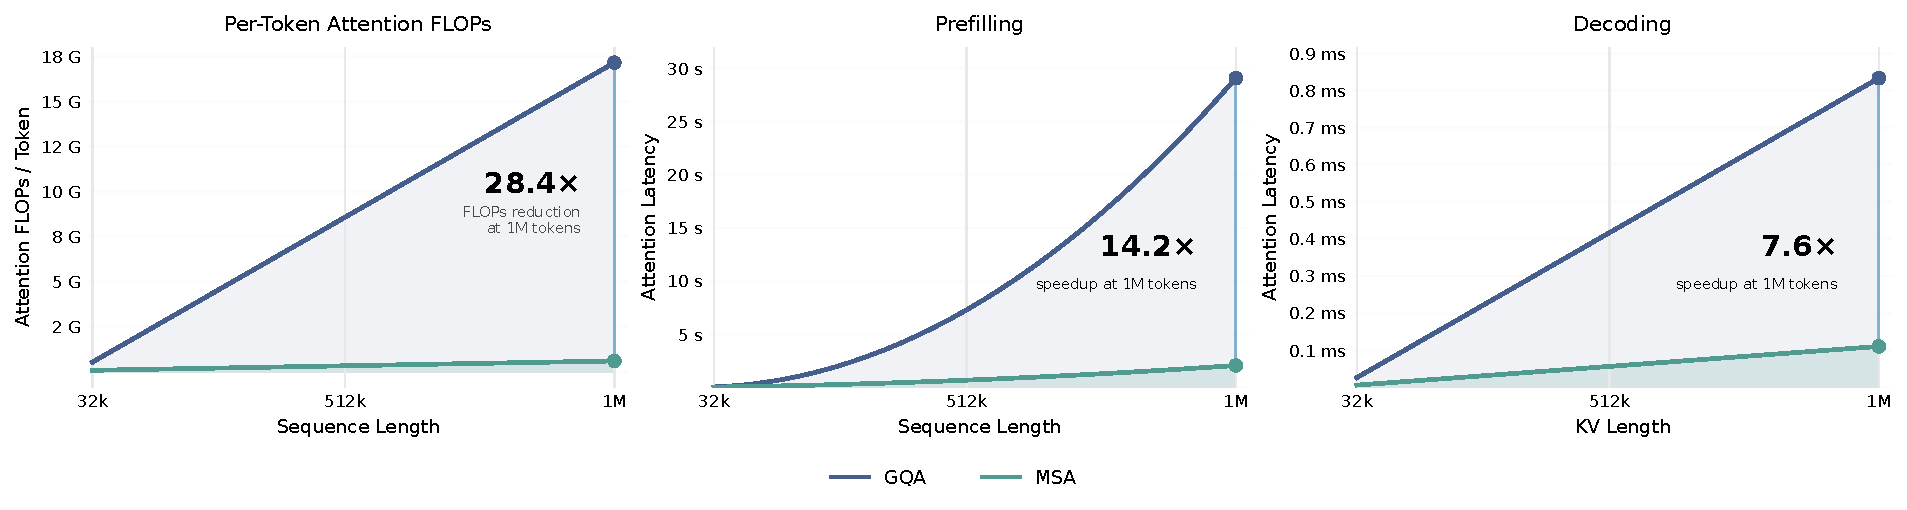
\includegraphics[width=0.98\linewidth]{figures/efficiency_gqa_vs_msa.pdf}
\caption{Efficiency comparison between GQA and \method{} under the shared experimental model configuration. The left subfigure reports the theoretical per-token attention-FLOPs. The middle and right subfigures report the measured implementation speedups for prefill and decode, respectively. All tests are conducted with 64 query heads, 4 key-value heads, and a head dimension of 128. \method{} uses $B_k=128$ and $k=16$, corresponding to a selected budget of $2{,}048$ tokens per query.}
\label{fig:efficiency}
\end{figure}
